\SubSection{Video Sampling Rate}

Macroblocks specify colors using a luminance channel to represent
saturation (color intensity), and two chrominance channels to
represent hue. The human eye is more sensitive to changes in
saturation than changes in hue, so the chrominance channels are
frequently compressed by downsampling the chrominance data within a
macroblock. The type of chrominance downsampling an MPEG-2 encoder
uses is its {\it chrominance format}. The most common chrominance
format is 4:2:0, which uses a single block for each of the chrominance
channels, downsampling each of the two channels from 16x16 to 8x8.
The other chrominance format with downsampling is 4:2:2, which uses
two blocks for each chrominance channel, downsampling each of the
channels from 16x16 to 8x16. The possible chrominance formats are
shown in Figure~\ref{fig:chroma-format}.

% TODO: Not sure if this goes here, at least change spacing and all that,
% but wanted to put it somewhere in the file.
\begin{figure}
  \begin{center}
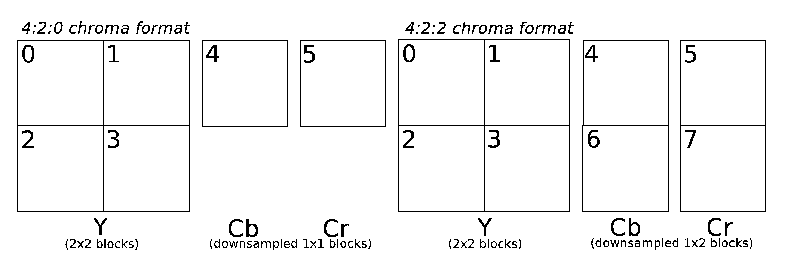
\epsfig{file=chroma_format.eps, width=3in}
% TODO change Matt's 3 am caption
% TODO let me know if you want me to show the 4:4:4 format as well, it wouldn't
% be too hard to generate it, but since we don't talk about it at all in the paper
% I didn't include it.
\caption{4:2:0 and 4:2:2 chrominance formats showing macroblock ordering}
\label{fig:chroma-format}
  \end{center}
\end{figure}

To support the 4:2:2 chrominance format in our StreamIt decoder, we
modified 31 lines and added 20 new lines. Of the 31 modified lines, 23
were trivial modifications to pass a variable representing the
chrominance format as a stream parameter. The greatest substantial
change was to the decoding splitjoin previously illustrated in
Figure~\ref{fig:decoding-sj}. The stream is reconfigured such that it
can properly deal chrominance data when the sampling rate is increased. 
Another change required to support the 4:2:2 chrominance format is the
interleaving of the chrominance data. As Figure~\ref{fig:chroma-format}
shows, only the luminance data always occurs in sequential macroblocks.
The chrominance data alternates between each of the two chrominance channels. 
To support this interleaving, the splitjoin responsible for parallel 
processing of the color channels is replaced by two nested splitjoins, shown in Figure~\ref{fig:chroma-stream}.

\begin{figure*}[t]
  \begin{scriptsize}
    \begin{verbatim}
    int->int splitjoin(int chromaFormat) {
      int xUpSample, yUpSample;

      if (chromaFormat == 420) { // 4:2:0 chroma format
        split roundrobin(4*N, 2*N);
	  xUpSample = yUpSample = 2;
      } else {                   // 4:2:2 chroma format
        split roundrobin(4*N, 4*N);
	  xUpSample = 2;
	  yUpSample = 0;
      }

      add LuminanceChannel(W, H, 0, 0, chromaFormat);

      add int->int splitjoin {
        split roundrobin(N, N);
        add ChrominanceChannel(W, H, xUpsample, yUpSample, chromaFormat);
        add ChrominanceChannel(W, H, xUpsample, yupsample, chromaFormat);
        join roundrobin(1, 1);
      }

      join roundrobin(1, 2);
  }
  \end{verbatim}
  \end{scriptsize}
  % \vspace{-3pt}
  \caption{Decoding stream to handle 4:2:0 and 4:2:2 chroma formats.}
  \label{fig:chroma-stream}
\end{figure*}



